\section{Wästlund 的构造}\label{sec:wastlund}

\subsection{亮度与平方反比}

点光源向各方向均匀发光，观察者在垂直于入射方向的小面上接收。距离为 $r$ 时，
同样的光通量摊在面积为 $4\pi r^{2}$ 的球面上，所以单位面积的亮度为
\begin{equation}
  B(r)=\frac{L}{4\pi r^{2}}\propto\frac{1}{r^{2}}.
  \label{eq:inverse-square}
\end{equation}
距离翻倍，亮度只剩四分之一。全文都把灯到观察点 $P$ 的距离代入这一式子，
因此 $\sum\frac{1}{d^{2}}$ 读起来就是 $P$ 处的总亮度。

\begin{definition}[灯、亮度与等效]\label{def:lamps}
平面上取定一点 $P$，称为\emph{观察点}。一盏\emph{灯}是某个 $Q\neq P$ 处的点光源，
它在 $P$ 处的\emph{亮度}就是数量 $\frac{1}{PQ^{2}}$；有限盏或可数盏灯的\emph{总亮度}
是各自亮度之和。若 $\frac{1}{PS_{1}^{2}}+\frac{1}{PS_{2}^{2}}=\frac{1}{PR^{2}}$，
就说两盏灯 $S_{1},S_{2}$（在 $P$ 处）\emph{等效于}一盏灯 $R$。
若过 $P$ 的圆以 $O$ 为圆心，则该圆上与 $P$ 直径相对的点称为 $P$ 的\emph{正对面}。
\end{definition}

有了这套说法，把一盏灯换成两盏等效灯就不改变总亮度，
需要核验的只剩反勾股恒等式，即引理 \ref{lem:inverse-pythagoras}。

\subsection{反勾股定理}

\begin{lemma}[反勾股]\label{lem:inverse-pythagoras}
设直角三角形的两条直角边为 $a,b$，斜边为 $c$，斜边上的高为 $h$，则
\begin{equation}
  \frac{1}{h^{2}}
  =\frac{c^{2}}{a^{2}b^{2}}
  =\frac{a^{2}+b^{2}}{a^{2}b^{2}}
  =\frac{1}{a^{2}}+\frac{1}{b^{2}}.
  \label{eq:inverse-pythagoras}
\end{equation}
\end{lemma}

\begin{proof}
两种面积表达式给出 $ab=ch$，于是 $c^{2}h^{2}=a^{2}b^{2}$；再代入 $c^{2}=a^{2}+b^{2}$
即得式 \eqref{eq:inverse-pythagoras}。
\end{proof}

\begin{figure}[htbp]
\centering
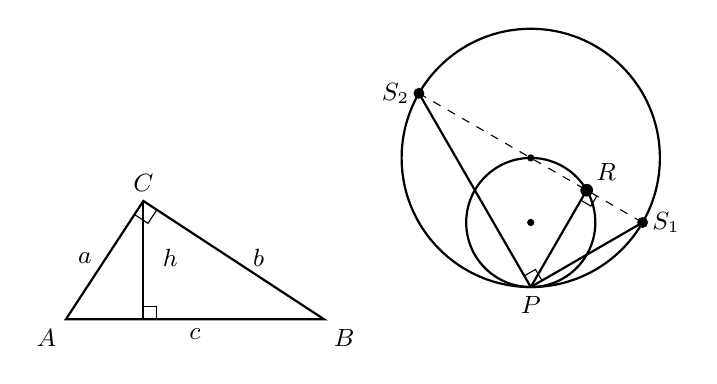
\begin{tikzpicture}[scale=0.82, every node/.style={font=\small}]
  \begin{scope}
    \coordinate (A) at (0,0);
    \coordinate (B) at (4,0);
    \coordinate (C) at (1.2,1.833);
    \coordinate (H) at (1.2,0);
    \draw[thick] (A)--(B)--(C)--cycle;
    \draw[thick] (C)--(H);
    \draw (1.4,0)--(1.4,0.2)--(1.2,0.2);
    \draw (1.063,1.624)--(1.272,1.487)--(1.409,1.696);
    \node[left] at (0.55,0.95) {$a$};
    \node[right] at (2.75,0.95) {$b$};
    \node[right] at (1.35,0.95) {$h$};
    \node[below] at (2,0) {$c$};
    \node[below left] at (A) {$A$};
    \node[below right] at (B) {$B$};
    \node[above] at (C) {$C$};
  \end{scope}

  \begin{scope}[shift={(7.2,0.5)}]
    \coordinate (P) at (0,0);
    \coordinate (O1) at (0,1);
    \coordinate (O2) at (0,2);
    \draw[thick] (O1) circle (1);
    \draw[thick] (O2) circle (2);
    \coordinate (R) at (0.866,1.5);
    \coordinate (S1) at (1.732,1);
    \coordinate (S2) at (-1.732,3);
    \draw[dashed] (S2)--(S1);
    \draw[thick] (P)--(R);
    \draw[thick] (P)--(S1);
    \draw[thick] (P)--(S2);
    \fill (R) circle (2.8pt);
    \fill (S1) circle (2.4pt);
    \fill (S2) circle (2.4pt);
    \fill (O1) circle (1.6pt);
    \fill (O2) circle (1.6pt);
    \draw (0.776,1.344)--(0.932,1.254)--(1.022,1.410);
    \draw (0.173,0.1)--(0.073,0.273)--(-0.1,0.173);
    \node[above right] at (R) {$R$};
    \node[right] at (S1) {$S_1$};
    \node[left] at (S2) {$S_2$};
    \node[below] at (P) {$P$};
  \end{scope}
\end{tikzpicture}
\caption{左：反勾股定理。右：引理 \ref{lem:replacement} 的替换。}
\label{fig:circle-replacement}
\end{figure}

\subsection{一盏灯换成两盏等效灯}

\begin{lemma}[替换]\label{lem:replacement}
设圆 $C_{1},C_{2}$ 的半径分别为 $r_{1}$ 与 $r_{2}=2r_{1}$，相切于观察点 $P$，
$R$ 是 $C_{1}$ 上的一盏灯。过 $R$ 作 $PR$ 的垂线，交 $C_{2}$ 于 $S_{1},S_{2}$，则
\begin{equation}
  \underbrace{\frac{1}{PR^{2}}}_{C_{1}\text{ 上一盏灯}}
  \;=\;
  \underbrace{\frac{1}{PS_{1}^{2}}+\frac{1}{PS_{2}^{2}}}_{C_{2}\text{ 上两盏灯}}.
  \label{eq:replacement}
\end{equation}
\end{lemma}

\begin{proof}
$C_{1}$ 上与 $P$ 直径相对的点在连心线上，到 $P$ 的距离是 $2r_{1}=r_{2}$，
所以它正是 $C_{2}$ 的圆心 $O_{2}$。因为 $PO_{2}$ 是 $C_{1}$ 的直径，角 $PRO_{2}$ 是直角：
过 $R$ 垂直于 $PR$ 的直线就是 $RO_{2}$，它在 $C_{2}$ 上截出的是一段直径的两个端点。
于是 $S_{1}S_{2}$ 是 $C_{2}$ 的直径，而 $P$ 在 $C_{2}$ 上，所以角 $S_{1}PS_{2}$ 是直角，
$PR$ 恰是它斜边上的高。把引理 \ref{lem:inverse-pythagoras} 用于三角形 $PS_{1}S_{2}$，
得到的正是式 \eqref{eq:replacement}。
\end{proof}

换句话说，小圆上的一盏灯可以换成大圆上的两盏灯，而 $P$ 处的亮度不变。

\subsection{翻倍：$N$ 等分点换成 $2N$ 等分点}

\begin{lemma}[翻倍]\label{lem:doubling}
在 $C_{1}$ 的 $N$ 个等分点各放一盏灯，逐盏按引理 \ref{lem:replacement} 换成 $C_{2}$ 上的像。
这些像正是与它们\emph{对应的} $C_{2}$ 的 $2N$ 等分点，且 $P$ 处的总亮度不变。
\end{lemma}

\begin{proof}
一盏灯 $R$ 的像是一对点，即过 $R$ 与 $O_{2}$ 的直径的两端，于是整幅图就是一束过 $O_{2}$ 的射线。
因为 $O_{2}$ 在 $C_{1}$ 上，相邻射线之间的角是 $C_{1}$ 上等弦所对的圆周角，两两相等；
同一批角又是 $C_{2}$ 的圆心角，所以射线与 $C_{2}$ 交出的 $2N$ 个点把 $C_{2}$ 等分。
亮度逐盏守恒，由引理 \ref{lem:replacement} 给出。
\end{proof}

「对应的」三个字要紧：这 $2N$ 个点是 $N$ 盏灯逐盏产生的，
任意取一组 $2N$ 等分点并不保持亮度。

\begin{figure}[htbp]
\centering
\begin{tikzpicture}[scale=0.78, every node/.style={font=\small}]
  \coordinate (P) at (0,0);
  \coordinate (O1) at (0,1);
  \coordinate (O2) at (0,2);
  \draw[thick] (O1) circle (1);
  \draw[thick] (O2) circle (2);
  \coordinate (R1) at (0.5,1.866);
  \coordinate (R2) at (0.5,0.134);
  \coordinate (R3) at (-1,1);
  \foreach \a [evaluate=\a as \c using {\a+180}] in {45,105,165}
    \draw[thin] ($(O2)+(\a:2)$)--($(O2)+(\c:2)$);
  \draw[thin] (P)--(R1);
  \draw[thin] (P)--(R2);
  \draw[thin] (P)--(R3);
  \foreach \a in {45,105,165,225,285,345}
    \fill[lampB] ($(O2)+(\a:2)$) circle (2.6pt);
  \fill[lampA] (R1) circle (3.2pt);
  \fill[lampA] (R2) circle (3.2pt);
  \fill[lampA] (R3) circle (3.2pt);
  \fill (O1) circle (1.3pt);
  \fill (O2) circle (1.3pt);
  \node[above left] at ($(O2)+(-0.24,0.24)$) {$O_2$};
  \node[below] at (P) {$P$};
\end{tikzpicture}
\caption{小圆的 $3$ 等分点换成大圆上对应的 $6$ 等分点。}
\label{fig:doubling}
\end{figure}

\subsection{极限：圆变成直线}

取周长为 $2$ 的圆，即半径 $R_{0}=\frac{1}{\pi}$，唯一的灯摆在 $P$ 的正对面。
它到 $P$ 的距离是 $\frac{2}{\pi}$，所以 $P$ 处的总亮度为
\begin{equation}
  \frac{1}{d^{2}}=\frac{1}{(2/\pi)^{2}}=\frac{\pi^{2}}{4}.
  \label{eq:first-lamp}
\end{equation}

\begin{figure}[H]
\centering
\begin{tikzpicture}[scale=0.78, every node/.style={font=\small}]
  \draw[dashed] (0,0)--(0,4);
  \draw[thick] (0,0.5) circle (0.5);
  \draw[thick] (0,1) circle (1);
  \draw[thick] (0,2) circle (2);
  \draw[thin,dashed] (-1,1)--(1,1);
  \draw[thin,dashed] (1.414,0.586)--(-1.414,3.414);
  \draw[thin,dashed] (-1.414,0.586)--(1.414,3.414);
  \fill[lampB] (1.414,0.586) circle (2.6pt);
  \fill[lampB] (-1.414,0.586) circle (2.6pt);
  \fill[lampB] (1.414,3.414) circle (2.6pt);
  \fill[lampB] (-1.414,3.414) circle (2.6pt);
  \fill[lampB] (1,1) circle (2.8pt);
  \fill[lampB] (-1,1) circle (2.8pt);
  \fill[lampA] (0,1) circle (3.4pt);
  \fill (0,0) circle (1.8pt);
  \node[below left] at (0,0) {$P$};
  \draw[->,thick] (2.5,2)--(3.7,2);
  \node[above,font=\footnotesize] at (3.1,2) {$k\to\infty$};
  \begin{scope}[shift={(7.1,0)}]
    \draw[thick] (-3.4,0)--(3.4,0);
    \fill (0,0) circle (1.8pt);
    \node[above] at (0,0) {$P$};
    \foreach \x/\lab in {-2.8/-7,-2.0/-5,-1.2/-3,-0.4/-1,0.4/1,1.2/3,2.0/5,2.8/7} {
      \fill[lampB] (\x,0) circle (2.6pt);
      \node[below,font=\footnotesize] at (\x,-0.05) {$\lab$};
    }
  \end{scope}
\end{tikzpicture}
\caption{半径逐轮翻倍，极限下圆压成过 $P$ 的直线。}
\label{fig:doubling-limit}
\end{figure}

每次翻倍都保持这一总亮度，翻倍 $k$ 次之后，周长 $2^{k+1}$ 的圆上的灯落在离 $P$
弧长 $1,3,5,\dots$ 处。当 $k\to\infty$ 时圆趋于它在 $P$ 的切线，弦长趋于弧长，
灯就落在直线上的 $\pm1,\pm3,\pm5,\dots$（图 \ref{fig:doubling-limit}），于是
\begin{equation}
  2\left(1+\frac{1}{3^{2}}+\frac{1}{5^{2}}+\cdots\right)=\frac{\pi^{2}}{4},
  \label{eq:odd-limit}
\end{equation}
两边除以 $2$ 就证明了定理 \ref{thm:wastlund}。

\subsection{回到巴塞尔问题}

式 \eqref{eq:basel} 的偶数项是整体级数的 $\frac14$，配上式 \eqref{eq:odd-sum} 就有
\begin{equation}
  \resizebox{\textwidth}{!}{$
  \begin{array}{r*{21}{c}r}
    &1&&&+&\frac{1}{3^{2}}&&&+&\frac{1}{5^{2}}&&&+&\frac{1}{7^{2}}&&&+&\frac{1}{9^{2}}
    &&&+&\cdots&=\frac{\pi^{2}}{8}\\[14pt]
    S=&1&+&\frac{1}{2^{2}}&+&\frac{1}{3^{2}}&+&\frac{1}{4^{2}}&+&\frac{1}{5^{2}}
    &+&\frac{1}{6^{2}}&+&\frac{1}{7^{2}}&+&\frac{1}{8^{2}}&+&\frac{1}{9^{2}}
    &+&\frac{1}{10^{2}}&+&\cdots&\\[20pt]
    \frac{1}{4}S=&&&\frac{1}{2^{2}}&&&+&\frac{1}{4^{2}}&&&+&\frac{1}{6^{2}}
    &&&+&\frac{1}{8^{2}}&&&+&\frac{1}{10^{2}}&+&\cdots&
  \end{array}$}
  \label{eq:odd-even}
\end{equation}
于是 $S=\frac{\pi^{2}}{8}\cdot\frac{1}{1-\frac14}=\frac{\pi^{2}}{6}$。最后这一段计算，
正是下面的定理 \ref{thm:direct} 要避开的代数步骤：式 \eqref{eq:odd-even} 把 $S$ 换成了
$\frac34 S$，图上的信息也就跟着换成了它的奇数项子级数。
